\section{Experimental Uncertainties}
\label{sec:ExpSystematics}

%\indent Experimental systematics are estimated using a simultaneous fit of CR and the results extrapolated to the SR in a background only fit.  Variations on MC background yield and kinematics are determined by different object performance groups using a number of simulation based and data driven in-situ techniques.  A simultaneous fit to the CR gives the best fit value of the systematic parameter $\alpha$ and the systematic uncertainty associated with the background prediction in the SR. \\

\subsection{Uncertainties on the Jet Energy Scale and Jet Energy Resolution } 

\indent The two main uncertainties affecting jet measurements are the uncertainties from jet energy scale and jet energy resolution calibrations. The jet reconstruction and calibration process is described in section \ref{sec:reco:jets}.  Uncertainty in the calibration process leads to uncertainty in the calorimeter response. \\

\indent jet energy scale uncertainties are derived from different in-situ techniques by the ATLAS Jet/$\met$ group.  These techniques exploit the transverse momentum balance between a jet and a reference object such as a photon or a Z boson or another jet.\cite{JES_dijet, JES_ZGamma}.  The jet energy scale uncertainty depends on $\eta$ and $\pt$ of the jet.  Uncertainties related to jet flavor composition and pile-up are also included.  \\

\indent  The ttbar CR requires similar jet multiplicity and jet energy as the SR.  Therefore, much of the jet energy scale and jet energy resolution uncertainties are canceled out in the transfer factor between the CR and SR.  Even after the cancelations, the jet energy scale uncertainty contributes a $\sim 10$ percent uncertainty to background yields and is one the major systematic uncertainties in this analysis.  \\

%\indent jet energy scale Uncertainty can be parameterized as a combination of 77 nuisance parameters.  This full set of nuisance parameter was combined to give a set of only 4 nuisance parameters.  The distribution of jets showed no dependence on the choice of full or reduced parameter set. \\

\indent The fractional jet energy scale uncertainty as a function of $\eta$ and $\pt$ for 2016 data can be see in figure \ref{fig:sys:JES}. \\

\begin{figure}[!h]
\begin{center}
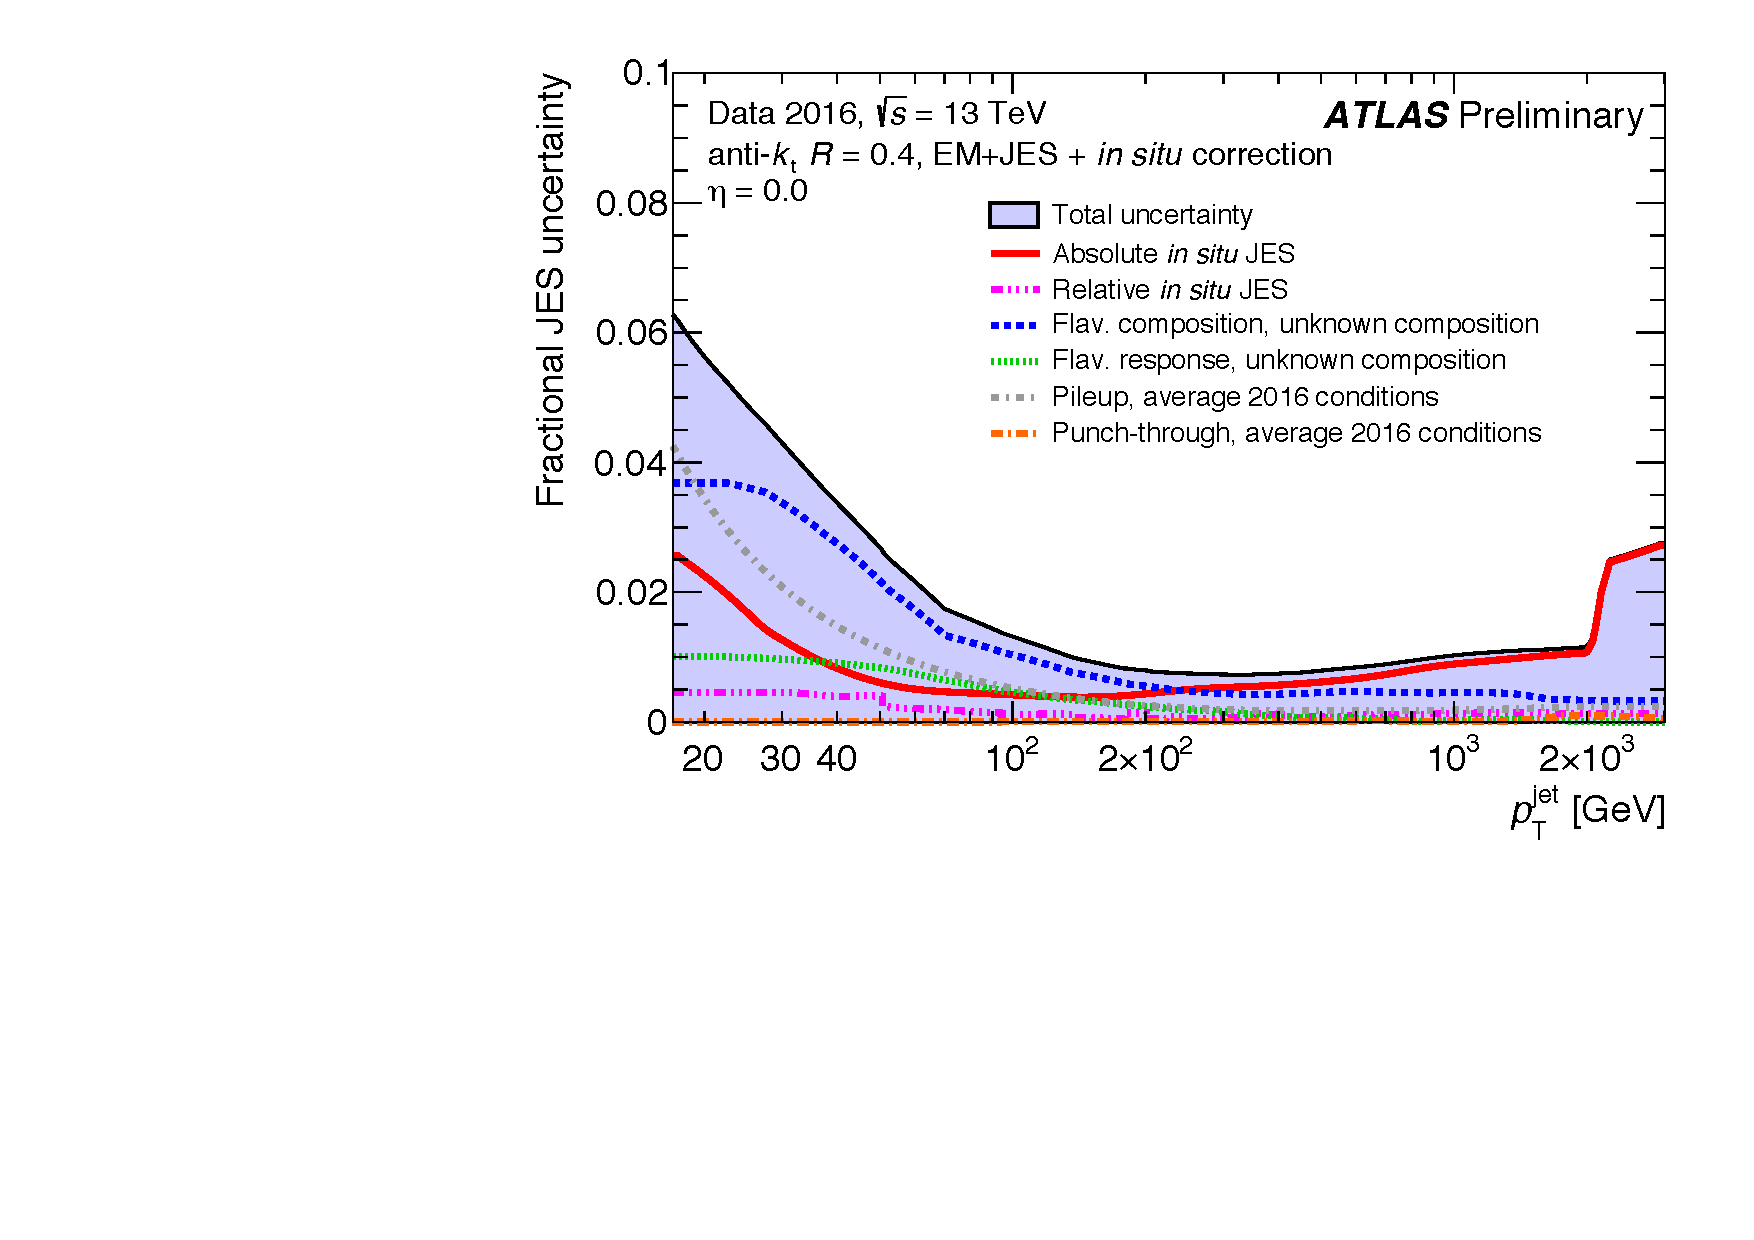
\includegraphics[width=0.55\textwidth, angle=270]{figures/JetCalib/JES_pt.pdf}
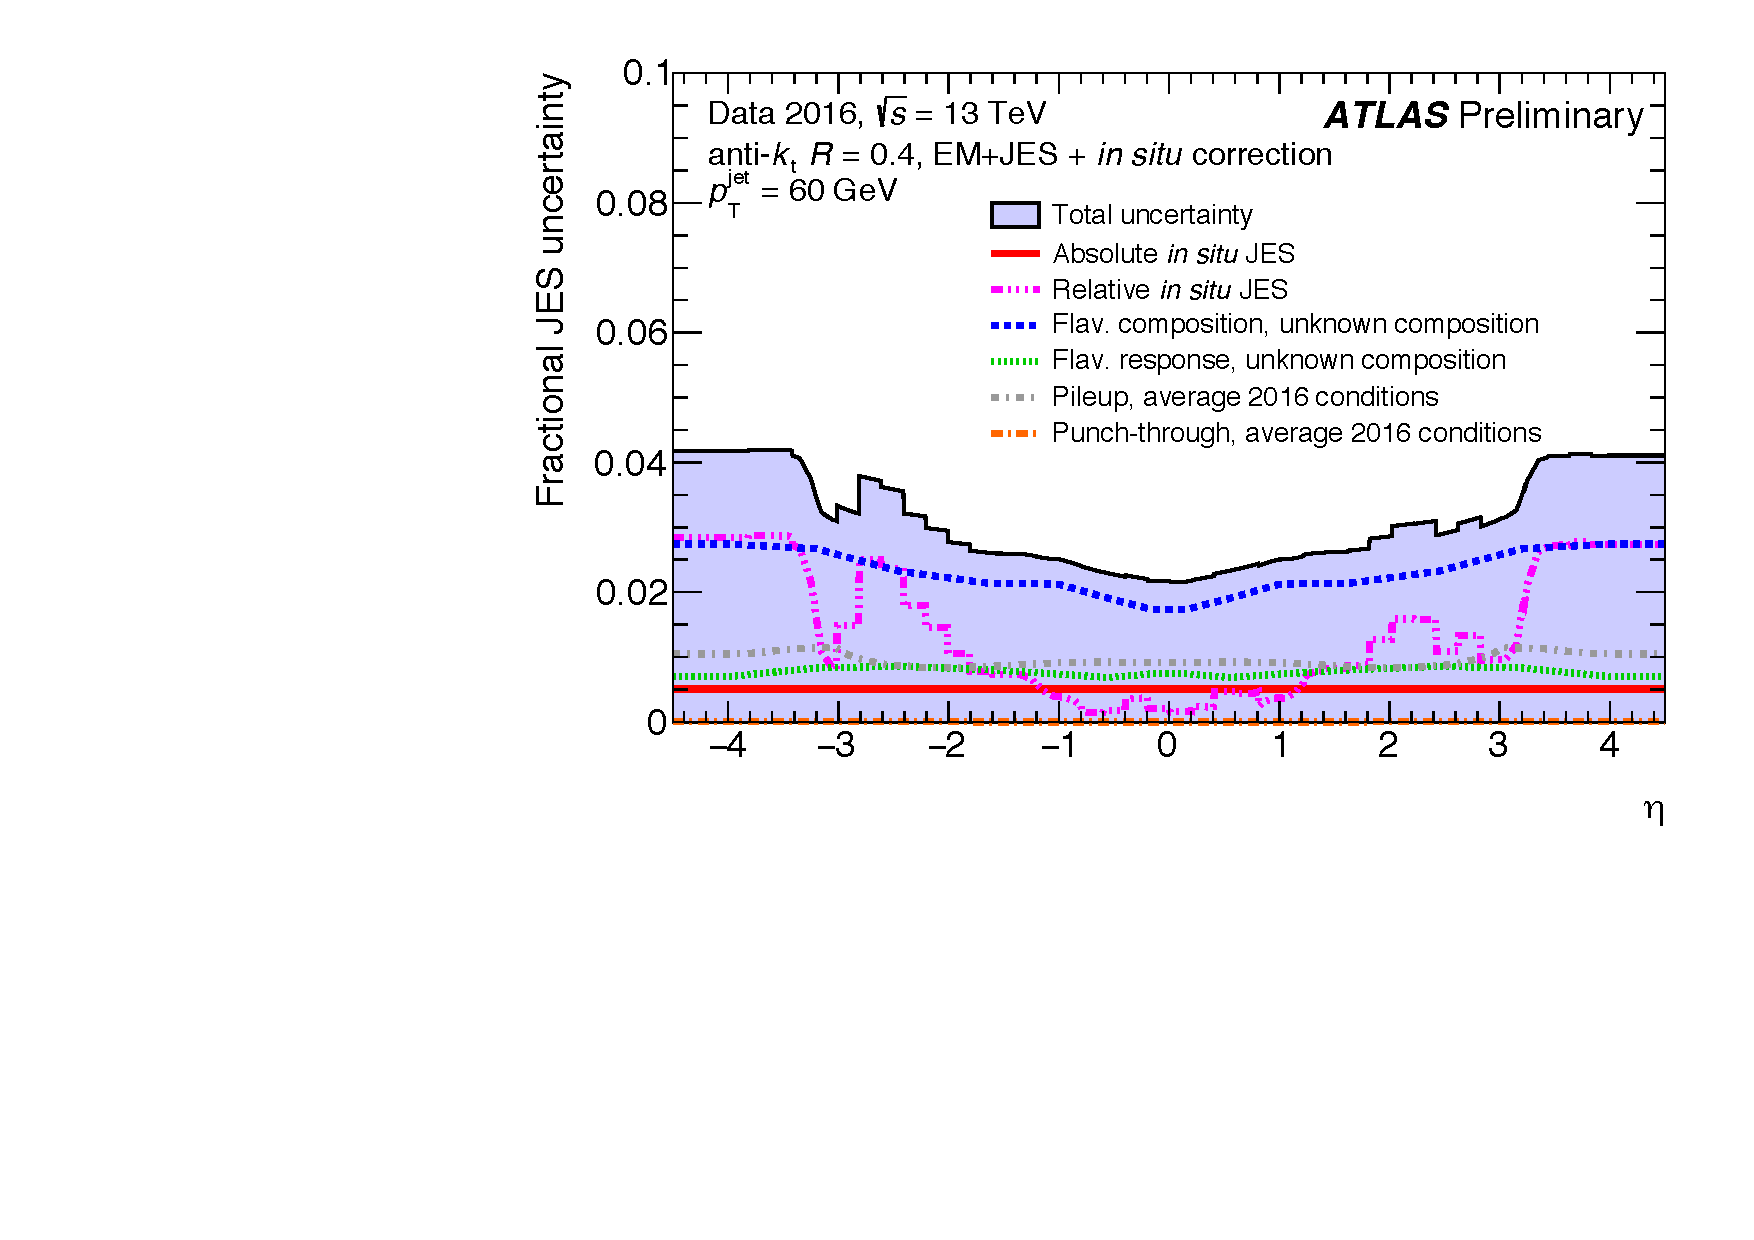
\includegraphics[width=0.55\textwidth, angle=270]{figures/JetCalib/JES_eta.pdf}
\caption[Fractional uncertainty on the jet energy scale vs jet $\eta$ and jet $\pt$. ]{Fractional uncertainty on the jet energy scale as a function of (a) jet $\eta$ and (b) jet $\pt$.  The jet energy resolution uncertainty depends on jet $\pt$, $\eta$ and $\phi$. Figure (a) is for central jets with $\eta = 0.0$.  Figure (b) is for jets with $\pt = 60 \gev$.  Both histograms are averaged over $\phi$ regions.}
\label{fig:sys:JES}
\end{center}
\end{figure}

\indent Uncertainties on the jet energy resolution are derived from dijet balance techniques.\cite{JES_dijet}  The fractional uncertainty on jet energy resolution as a function of $\eta$ and $\pt$ can be seen in figure \ref{fig:sys:JER}\\

\begin{figure}[!h]
\begin{center}
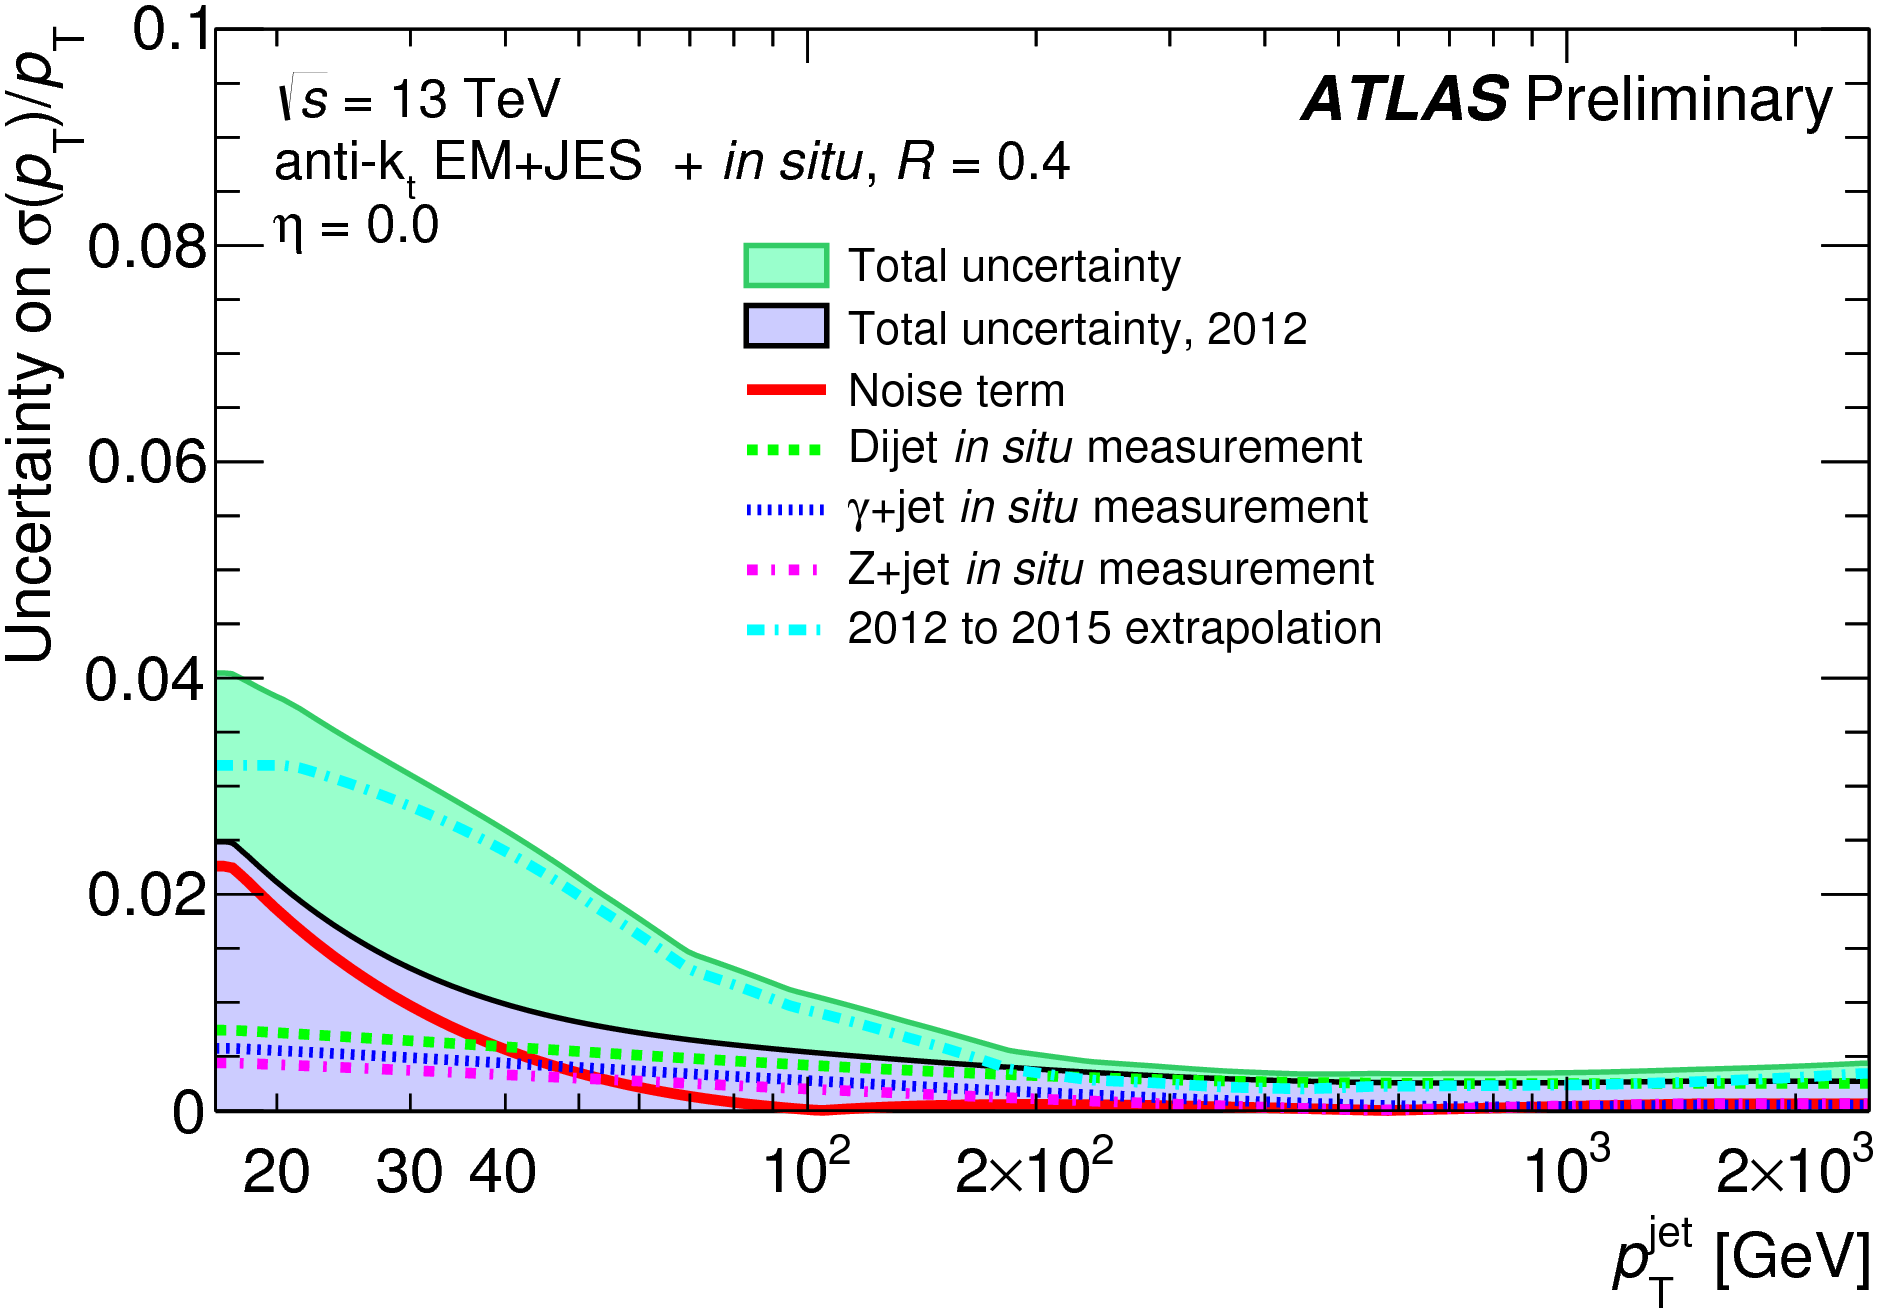
\includegraphics[width=0.85\textwidth]{figures/JetCalib/JER_pt.png}
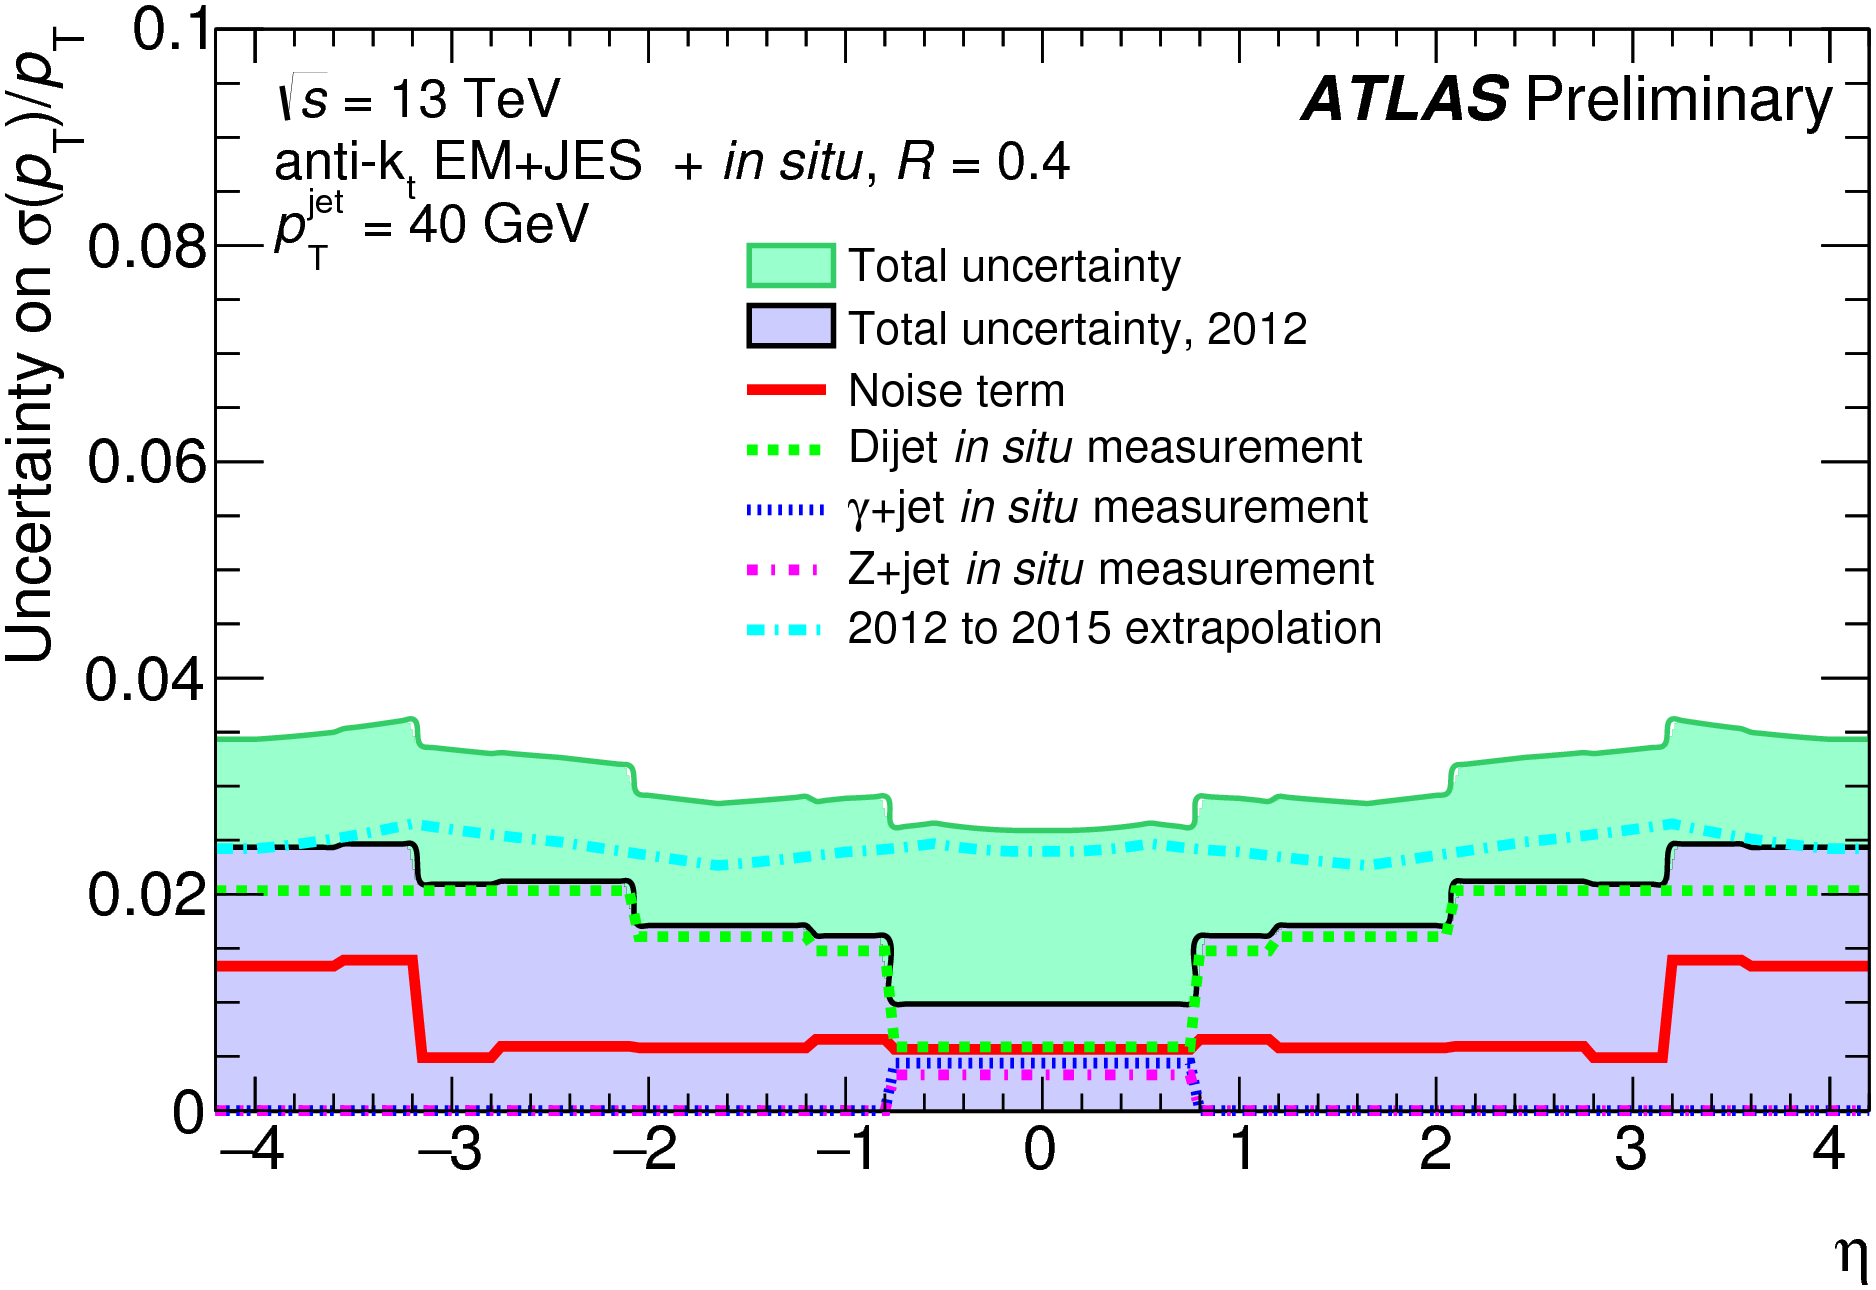
\includegraphics[width=0.85\textwidth]{figures/JetCalib/JER_eta.png}
\caption[Fractional uncertainty on the jet energy resolution as a function of jet $\eta$ and jet $\pt$.]{Fractional uncertainty on the jet energy resolution as a function of (a) jet $\eta$ and (b) jet $\pt$.  The jet energy resolution uncertainty depends on jet $\pt$, $\eta$ and $\phi$.  Figure (a) is for central jets with $\eta = 0.0$.  Figure (b) is for jets with $\pt = 40 \gev$.  Both histograms are averaged over $\phi$ regions. }
\label{fig:sys:JER}
\end{center}
\end{figure}

\subsection{Uncertainty on $b$-tagging Efficiency}

\indent  The $b$-tagging uncertainty is derived by the ATLAS flavor-tagging working group.  A separate set of weights are applied for each set of $b$-tagging variations.  These include scale factors on $b$-tagging efficiencies and the rate of mis-tagging of $c$-jets and light-flavored jets. The b-tagging efficiency uncertainty as a function of jet $\pt$ in ttbar is shown as the green shaded region in figure \ref{fig:sys:btag}. \\

\begin{figure}[!h]
\begin{center}
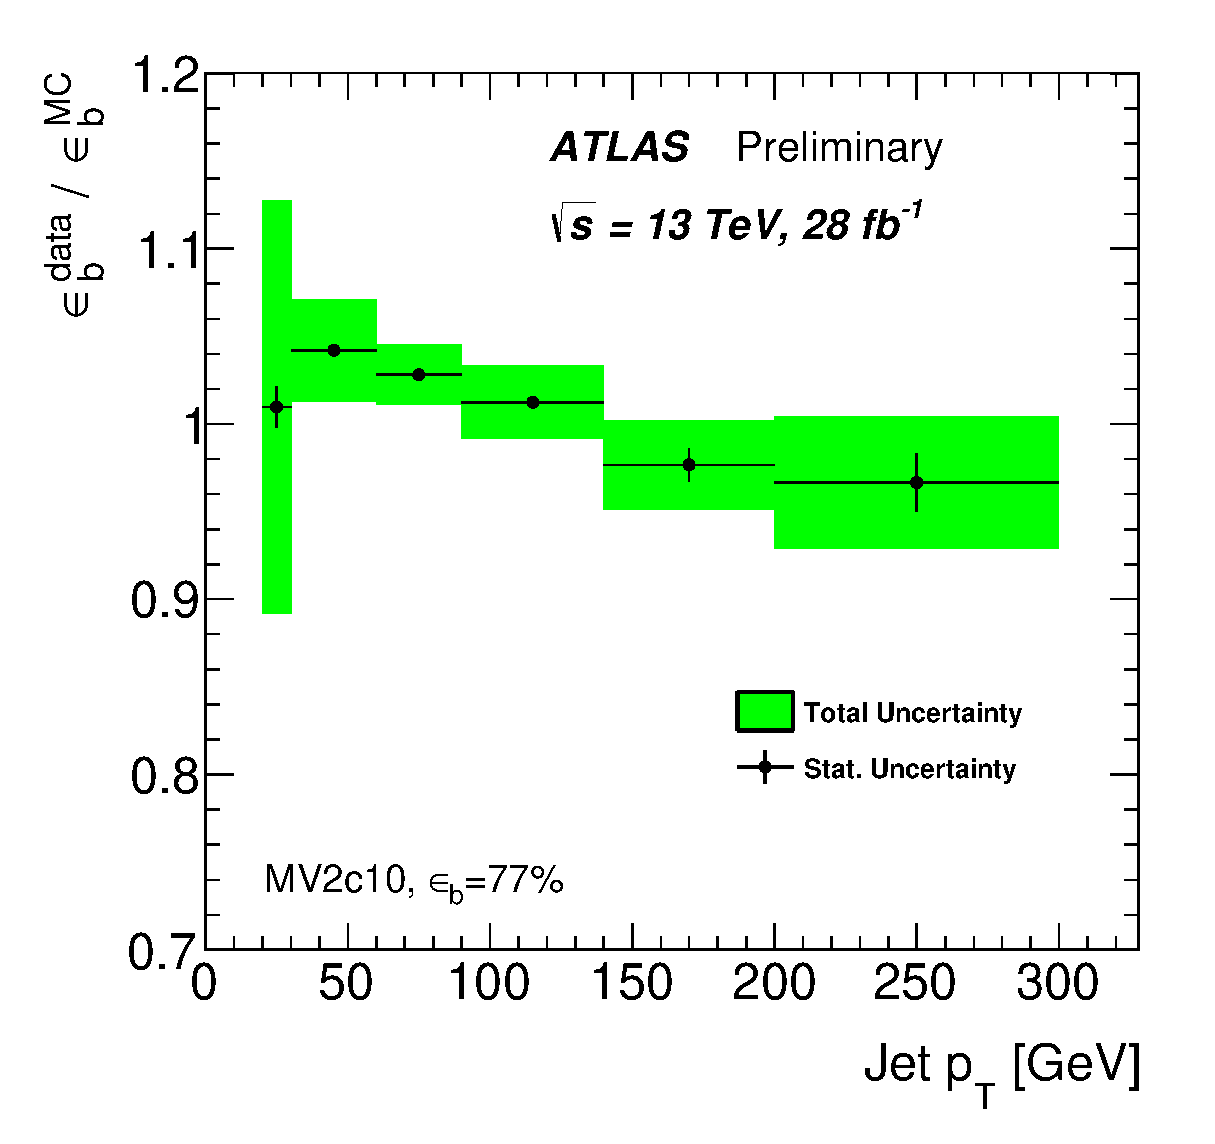
\includegraphics[width=0.85\textwidth]{figures/JetCalib/MV20c10_btaggingEff.eps}
\caption[Ratio of b-tagging efficiency in data and MC between data and MC.]{Ratio of b-tagging efficiency in data and Monte Carlo for the MV2c10 b-tagging algorithm at the 77\% working point as a function of jet $\pt$. The b-tagging efficiency was extracted from a ttbar enriched region. Statistical errors (black lines) and total errors (green shaded region) are shown. The bin below a $\pt$ of $30\gev$ has large uncertainties.}
\label{fig:sys:btag}
\end{center}
\end{figure}

\indent Uncertainties on $b$-tagging do not contribute a large systematic uncertainty to our analysis because we only require one b-tagged jet with $\pt > 40 \gev$.  Having a $\pt > 40 \gev$ requirement avoids the large uncertainty on $b$-tagging efficiency at low $\pt$.  

\indent At the same time, there is little extrapolation between background CRs and SR. The ttbar, $W$+jets and QCD multijets all use CRs that also require one $b$-tagged jet.  After fitting to CRs, $b$-tagging systematics amount to only a 1-3 percent uncertainty on the total background rate in SR.  \\

\subsection{Uncertainty on the $\met$ Soft Term}

\indent The $\met$ is defined in equation \ref{eqn:metReco1} as the negative vector sum of all hard reconstructed objects and a ``soft term''.  Hard objects include reconstructed electrons, photons, jets, and muons.  The soft term is determined by summing over the $\pt$ of all ID tracks that aren't associated with any hard objects and is intend to estimate all the energy not associated with any hard reconstructed objects.  Although the soft term only registers the $\pt$ from charged objects, it is able to effectively reject any energy deposited by pileup interactions because ID tracks can be associated with the hard interaction primary vertex. \\

\begin{equation}
\met = - ( \sum_{hard~objects} E_T + \sum_{soft} E_T ) 
\label{eqn:metReco1}
\end{equation}

\indent  The majority of the uncertainty on $\met$ has already been accounted for by systematics on other reconstructed objects because the $\met$ is built mostly out of fully calibrated and reconstructed physics objects.  However, the $\met$ soft term is independent from any hard physics object.  Therefore, uncertainty on the $\met$ soft term forms an independent systematic uncertainty.  \\

\indent The uncertainty on the resolution and scale of the $\met$ soft term is derived by the ATLAS Jet/$\met$ group using two in-situ methods using $Z\rightarrow \mu\mu$ events.\cite{METPerform} The uncertainty on the $\met$ track soft term (TST) vs the number of reconstructed primary vertexes in $\ttbar$ simulation is shown in figure \ref{fig:sys:MET_TST_tt}. \\

\begin{figure}[!htbp]
\begin{center}
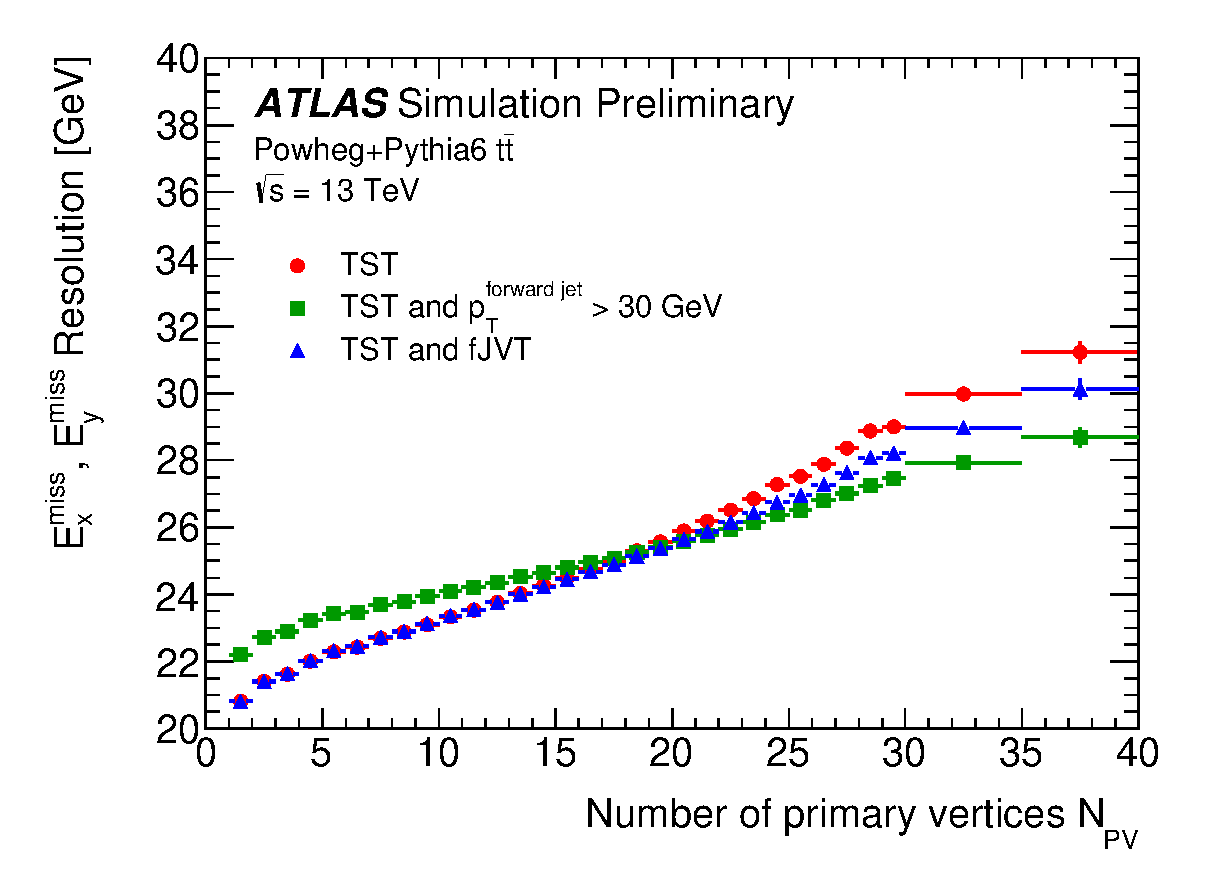
\includegraphics[width=0.48\textwidth]{figures/METCalib/MET_TST_tt.eps}
\caption[Uncertainty on the $\met$ track soft term as a function the number of reconstructed vertexes.]{Uncertainty on the $\met$ track soft term as a function the number of reconstructed vertexes.  More reconstructed vertexes means more pileup interactions are in the event. }
\label{fig:sys:MET_TST_tt}
\end{center}
\end{figure}

\indent The $\met$ soft term resolution and scale uncertainty contribute a $1-2\%$ uncertainty on the total background yield.  The small uncertainty result from the high $\met$ requirement of at least 250 $\gev$ and little to no extrapolation across $\met$ between CR and SR for all major backgrounds. \\

\subsection{Uncertainty on Lepton Reconstruction Efficiencies and Energy Scale}

\indent Uncertainty on lepton reconstruction and identification propagate to uncertainty on CR and SR yields.  These uncertainties include uncertainties on e/$\gamma$ resolution, energy scale, and reconstruction efficiency and muon momentum and reconstruction efficiency.  Lepton trigger scale factors are also taken into account for the $\ttbar+\gamma$ control region. \\

\indent These uncertainties are derived by the ATLAS E/$\gamma$ and muon combined performance groups and result in sub 1\% uncertainty on signal region yields.\cite{MuonReco,EleID} \\

\subsection{Pileup Uncertainty}

\indent The uncertainty on the amount of pileup in 2015 and 2016 ATLAS data is estimated using a two sided variation in event weights.  One set of weight simulate a lower rates of pile-up interactions and the other simulate a higher rate.  Pile-up uncertainty contributes a 1-2\% uncertainty on the total background yield in the SR.



  % The detector systematic uncertainties above are calculated as the variations in the shapes of the original normalized histograms using ${\tt overallNormHistoSys}$ inside ${\tt HistFitter}$.
% \item{\bf Luminosity}
%The uncertainty of 2.8 $\%$ is assigned for the integrated luminosity and is denoted by {\bf Lumi} in the fit.


  %%%%%%%%%%%%%%%%%%%%%%%%%%%%%%%%%%%%%%%%%%%%%%%%%%%%%%%%%%
  %% Commented out for the time being since the est, method are not fully defined yet
  %%%%%%%%%%%%%%%%%%%%%%%%%%%%%%%%%%%%%%%%%%%%%%%%%%%%%%%%%%
%% \item{\bf Z fit method for $Z+jets$ background}
%% Following the detailed study in Section~\ref{section:Z_Results}, the uncertainty of 17
%% $\%$ is assigned to $Z+jets$ background for the $Z+jets$ fit-method estimation and is denoted by {\bf methodSysZ} in the fit.

%% \item{\bf Jet-smearing estimation method for multi-jet background}
%% The uncertainty of 100 $\%$ to is conservatively assigned to the
%% multi-jet yields for the jet-smearing estimation method and is denoted by
%% {\bf theoSysQCD} in the fit.

%% \item{\bf \dphimettrk\ and tau veto}
%%   No additional uncertainty is assigned for the requirements on
%%   \dphimettrk\ and on the tau veto. Both were discussed extensively for
%%   the 7 \TeV\ analysis \cite{7TeVSupportNote} where no additional
%%   systematic was assigned.  There are currently no official
%%   recommendations from the jet/etmiss group for \mettrk.  For the 7
%%   \TeV\ analysis, Fig 42 in Appendix C showed good agreement between
%%   data and MC for \dphimettrk\ in the tau-veto-inverted validation
%%   region.  For the current analysis, Fig. \ref{fig:SRA_dataMC} shows
%%   good agreement for the \mettrk\ variables in a \ttbar\ dominated
%%   region.  Tau veto systematics are documented in Appendix D of the 7
%%   \TeV\ note.  Data/MC comparisons were made for several variables in
%%   the 1-lepton control region and in the tau-veto-inverted validation
%%   region.  The tau fake rate was determined in a $Z\nu\nu$+jets
%%   dominated sample to be around 12\%. The systematic on this fake rate
%%   was determined with a study of the track multiplicity in jets; the
%%   track multiplicity for ($n_{trk} \le 4$) showed agreement within 5\%
%%   between data and MC.

  %%%%%%%%%%%%%%%%%%%%%%%%%%%%%%%%%%%%%%%%%%%%%%%%%%%%%%%%%%
  %%%%%%%%%%%%%%%%%%%%%%%%%%%%%%%%%%%%%%%%%%%%%%%%%%%%%%%%%%
  

  
